\documentclass[conference]{IEEEtran}
\IEEEoverridecommandlockouts
% The preceding line is only needed to identify funding in the first footnote. If that is unneeded, please comment it out.
%Template version as of 6/27/2024

\usepackage{cite}
\usepackage{amsmath,amssymb,amsfonts}
\usepackage{algorithmic}
\usepackage{graphicx}
\usepackage{textcomp}
\usepackage{xcolor}
\setlength{\tabcolsep}{2pt}
\setlength{\arraycolsep}{2pt}
\def\BibTeX{{\rm B\kern-.05em{\sc i\kern-.025em b}\kern-.08em
    T\kern-.1667em\lower.7ex\hbox{E}\kern-.125emX}}


\DeclareMathOperator*{\argmax}{arg\,max}
\DeclareMathOperator*{\argmin}{arg\,min}
\DeclareMathOperator{\diag}{diag}

\begin{document}

\title{Centroidal MPC for Inertial Reorientation Using
Bio-inspired Tailed Robot}

\author{Yichen Wang, Qin Yue
}

\maketitle

\begin{abstract}
ABSTRACT ABSTRACT ABSTRACT ABSTRACT ABSTRACT ABSTRACT ABSTRACT ABSTRACT ABSTRACT ABSTRACT ABSTRACT ABSTRACT ABSTRACT ABSTRACT ABSTRACT ABSTRACT ABSTRACT ABSTRACT ABSTRACT ABSTRACT ABSTRACT ABSTRACT ABSTRACT ABSTRACT ABSTRACT ABSTRACT ABSTRACT ABSTRACT ABSTRACT ABSTRACT ABSTRACT ABSTRACT ABSTRACT ABSTRACT ABSTRACT ABSTRACT ABSTRACT ABSTRACT ABSTRACT ABSTRACT ABSTRACT ABSTRACT ABSTRACT ABSTRACT ABSTRACT ABSTRACT ABSTRACT ABSTRACT ABSTRACT ABSTRACT ABSTRACT ABSTRACT ABSTRACT ABSTRACT ABSTRACT ABSTRACT ABSTRACT ABSTRACT ABSTRACT ABSTRACT ABSTRACT ABSTRACT ABSTRACT ABSTRACT ABSTRACT ABSTRACT ABSTRACT ABSTRACT ABSTRACT ABSTRACT ABSTRACT ABSTRACT ABSTRACT ABSTRACT ABSTRACT ABSTRACT ABSTRACT ABSTRACT ABSTRACT ABSTRACT ABSTRACT ABSTRACT ABSTRACT ABSTRACT ABSTRACT ABSTRACT ABSTRACT ABSTRACT ABSTRACT ABSTRACT ABSTRACT ABSTRACT ABSTRACT ABSTRACT ABSTRACT ABSTRACT ABSTRACT ABSTRACT ABSTRACT ABSTRACT ABSTRACT ABSTRACT ABSTRACT ABSTRACT ABSTRACT 
\end{abstract}

% \begin{IEEEkeywords}
% component, formatting, style, styling, insert.
% \end{IEEEkeywords}

\section{Introduction}

Inertial reorientation (IR) refers to the ability of a robot to change its orientation without or with minimal interaction with the ground or other objects. This movement can increase robot agility by stabilizing the robot between ground contacts in gaits with long flight phases, rejecting sudden disturbances, or increasing the speed of the robots turns. A tail-like appendage is shown to be effective in increasing the robot's ability for inertial-reorientation \cite{libby2016tail}.

However, the addition of a tail appendage makes the robot system more complex. Moreover, effective inertial reorientation control frequently necessitates control using the full-body dynamic model of the robot, as opposed to the typical approach of abstracting the robot to a single rigid body. Centroidal MPC can represent a useful compromise of these two methods \cite{dai2014centroid}.


\section{Methods}

\begin{figure*}[t]
    \centering
    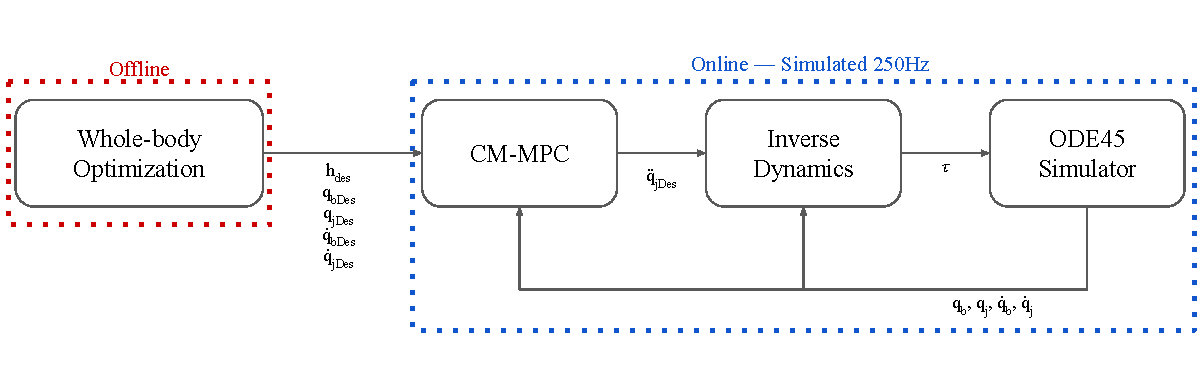
\includegraphics[width = \linewidth]{figures/system_graph.pdf}
    \caption{Illustration of the overall system. An offline trajectory optimization feeds reference trajectories into a simulated online CM-MPC and Inverse Dynamics controller to control the robot.}
    \label{fig:system}
\end{figure*}

\subsection{Robot Model}
We use a bipedal tailed robot model. The robot has eight actuated degrees of freedom, denoted $q_j \in \mathbb{R}^8 $: two for the tail, and three for each leg. The tail is modelled as two sequentially actuated joints for pitch and yaw, placed close to the torso, with a long bar and a heavy counterweight connected at the end. Each leg is modeled as three sequential joints for adduction-abduction, hip extension-flexion, and knee-extension-flexion. Additionally, the model includes six floating base joints, $q_b \in \mathbb{R}^6 $,  to simulate free movement in three dimensions: three linear joints in the x, y, and z direction, and three rotating joints in the x, y, and z axis.

\begin{figure}[h]
    \centering
    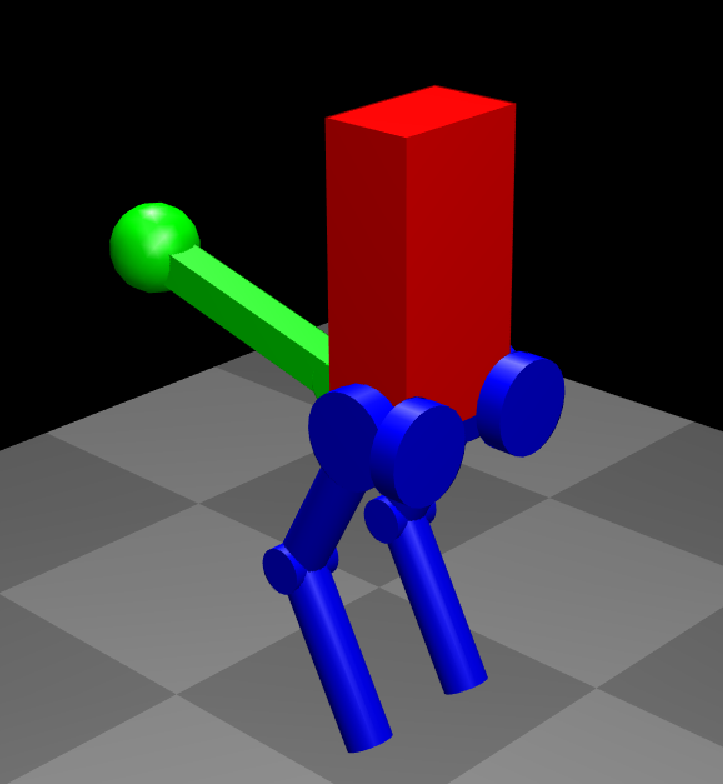
\includegraphics[height=0.45\linewidth]{figures/robot_model.png}
    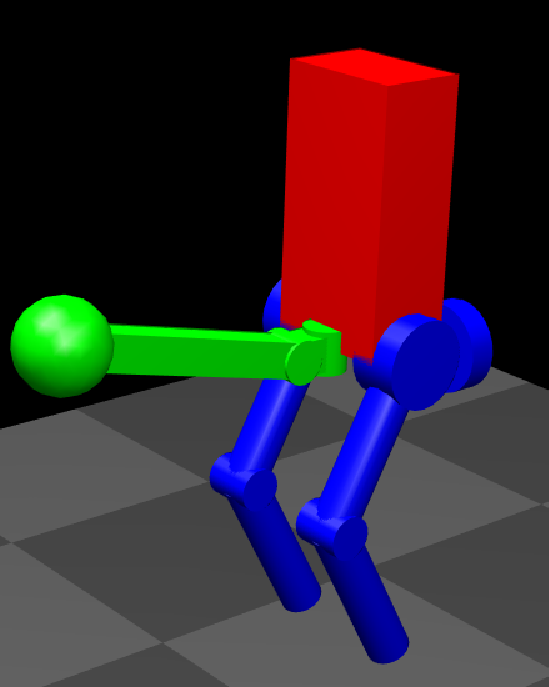
\includegraphics[height=0.45\linewidth]{figures/robot_back.png}
    \caption{Robot model with $q_j =$ [0 .25 0 .5 -1 0 .5 -1]$^\top$}
    \label{fig:robotmodel}
\end{figure}

We used the software package Spatial V2 \cite{featherstone2008spatialv2} to model and visualize this model, shown in figure \ref{fig:robotmodel}. The parent link, joint properties, mass, and inertia of each link are denoted in Table \ref{tab:robotparams}, where $p(j)$ denotes the parent link of link $i$, Position denotes the translation portion of the transform from the predecessor frame to the current link frame, $^i \mathbf{X}_p(i)$, CoM Pos refers to the center of mass postion in the current link frame, $I \in \mathbb{R}^{3 \times 3}$ refers to the diagonalized link inertia around the CoM. All link frames are constructed with identical orientation to the world frame when $q_j = \mathbf{0}^8$, so frame orientations are ommitted. Link 0, or the Torso, is connected to ground via six sequential floating-base joints, using the order $\begin{bmatrix}
    Px & Py & Pz & Rx & Ry & Rz
\end{bmatrix}$. $q_b$ and $q_j$ are constructed with the same order as above. 
\vspace{-5mm}
\begin{table}[h]
    \centering
    \caption{Table of robot Parameters.  }
    \begin{tabular}{|c | c| c |c| c| c| c| c|}
        \hline
        $i$ & Name & $p(i)$ & Axis & Frame Pos.& M & CoM Pos. & diag$(I) \times 10^4$ \\
        \hline
        \hline
        0 & Torso & n/a & n/a & [0 0 0] & 1 & [0 0 .2]& [94 83 27]\\
        1 & Tail-Y & 0 & z & [-0.05, 0, 0] & .05 & [-0.025  0  0]& [0    0.104    0.104]\\
        2 & Tail-P & 1 & y & [-0.05, 0, 0] & .5 & [-0.27  0  0]& [0    25.5    25.5]\\
        3 & AbAd-R & 0 & x & [0, -.075, 0] & .3 & [0 0 0] & [0.625 22.75 22.75]\\
        4 & Hip-R & 3 & y & [0, 0, 0] & .75 & [0 0 -0.02]& [18.25 38.8 21.8]\\
        5 & Knee-R & 4 & y & [0, 0, -0.2] & .1 & [0 0 -0.1]& [3.33 3.33 0]\\
        6 & AbAd-L & 0 & x & [0, .075, 0] & .3 & [0 0 0] & [0.625 22.75 22.75]\\
        7 & Hip-L & 6 & y & [0, 0, 0] & .75 & [0 0 -0.02]& [18.25 38.8 21.8]\\
        8 & Knee-L & 7 & y & [0, 0, -0.2] & .1 & [0 0 -0.1]& [3.33 3.33 0]\\
        \hline
    \end{tabular}
    {\raggedright  \par}
    \label{tab:robotparams}
\end{table}
\vspace{-5mm}

Simulation is done using a discretized model and the \texttt{ode45} \cite{shampine1997matlab} function supplied with MATLAB. Specifically, we use a zero-order hold on the inputs, then simulate the system forward until the end of the time step. The state is then updated to the final state of the simulation, and the simulation repeated with more inputs generated from the centroidal MPC.

\subsection{Trajectory Optimization Formulation}

Reference trajectories for online CM-MPC controller are generated using offline trajectory optimization. We formulated the trajectory optimization problem as an NLP, shown as follows

\begin{align}
    &\argmin_{x, \dot{x}, \tau} \sum^{N_{hor}-1}_{n=1} \tau^\top \diag(w_1) \tau + \varepsilon_x^\top \diag(w_2) \varepsilon_x \\
     \text{subject to} & \nonumber \\
     \varepsilon_x & = x_n - x_{des, n} \\
    x_{n+1} & =\ddot{x}_n(x_n,\dot{x}_n, u) \\
    x_n &< \text{UB} \\
    x_n &> \text{LB}
\end{align}



\subsection{Centroidal Matrix Formulation}

The centroidal momentum, $h_G \in \mathbb{R}^6$ of a robot refers to the sum of all link momenta, projected to the center of mass frame of the robot \cite{orin2008centroidal}. We will first define the concatenated spatial velocity of all links as $v = \left[ \begin{matrix}
    v_1 & v_2 & \dots & v_8 \end{matrix}\right]^\top$, and the spatial velocity of a specific link as $v_i \in \mathbb{R}^6$, and find the relation

\begin{equation}
    v_i = \begin{bmatrix}
        \omega_i \\ \nu_i
    \end{bmatrix} = ^i \mathbf{X}_p(i) v_{p(i)} + \mathbf{\Phi}_i \dot{q}_i
    \label{eq:vi}
\end{equation}
where $\omega_i \in \mathbb{R}^3$ is the angular velocity, $\nu_i \in \mathbb{R}^3$ is the linear velocity, and $\mathbf{\Phi}_i \in \mathbb{R}^6$ is the motion subspace matrix, which selects the axis in which a joint acts on. For example, a revolute joint in the y direction has $\mathbf{\Phi}_{Ry} = \left[ \begin{matrix}
0 & 1 & 0 & 0 & 0 & 0 \end{matrix}\right]^\top$.

We can shuffle (\ref{eq:vi}) to get (\ref{eq:vi2}), the difference of velocity between a link and its predecessor. 
\begin{equation}
    v_i - ^i \mathbf{X}_p(i) v_{p(i)} = \mathbf{\Phi}_i \dot{q}_i
    \label{eq:vi2}
\end{equation}

Then, we find the relationship between $v$ and $\dot{q}$ to be
\begin{align}
    P v &=  \mathbf{\Phi} \dot{q} \\
    P_{ij} &= \begin{cases}
        \mathbf{1}^{6\times 6}&, j = i\\
        - ^i \mathbf{X}_p(i) v_{p(i)}&, j = p(i) \\
        \mathbf{0}^{6\times 6} &, \text{else} \\
    \end{cases} \\
    \mathbf{\Phi} &= \begin{bmatrix}
        \mathbf{\Phi}_1 & \mathbf{0}^{6} & \dots & \mathbf{0}^{6} \\
        \mathbf{0}^{6} & \mathbf{\Phi}_2 & \dots  & \mathbf{0}^{6} \\
        \vdots & \vdots & \ddots & \vdots\\
        \mathbf{0}^{6} &\mathbf{0}^{6} &\dots & \mathbf{\Phi}_8
    \end{bmatrix}
\end{align}

where $P \in \mathbb{R}^{48\times 48}$ is a nonstandard incidence matrix, and $\mathbf{\Phi} \in \mathbb{R}^{48 \times 8}$ is the diagonalized joint selection matrix.

We can also find the relation $h = I v$ between $h \in \mathbb{R}^{48}$, the system momentum matrix and $I \in \mathbb{R}^{48 \times 48}$, with
\begin{align}
    h & = \begin{bmatrix}
        h_1 \\ h_2 \\ \vdots \\ h_8
    \end{bmatrix} \\
    I & = \begin{bmatrix}
        I_1 & \mathbf{0}^{6} & \dots & \mathbf{0}^{6} \\
        \mathbf{0}^{6} & I_2 & \dots  & \mathbf{0}^{6} \\
        \vdots & \vdots & \ddots & \vdots\\
        \mathbf{0}^{6} &\mathbf{0}^{6} &\dots & I_8
    \end{bmatrix}
\end{align}
where $h_i \in \mathbb{R}^6 $ is the link momentum in the world frame, and $I_i \in \mathbb{R}^{6 \times 6}$ is the link inertia. In order to find the centroidal momentum, we must transform the link momentum from the world frame into the CoM frame, and then sum it

\begin{equation}
    h_G = \sum^8_{i=1} {}^i\mathbf{X}^T_G h_i = \sum^8_{i=1} {}^i\mathbf{X}^T_G I_i v_i
\end{equation}
Using matrix manipulation to subsitute the summation, we find
\begin{equation}
    h_G = \mathbf{X}^T_G I P^{-1} \mathbf{\Phi} \dot{q}
    \label{eq:hg}
\end{equation}
where $\mathbf{X}$ is the projection matrix from centroidal coordiantes to all link coordiantes,
\begin{equation}
    \mathbf{X}_G = \begin{bmatrix}
        ^1X_G^\top\\
        ^2X_G^\top\\
        \vdots \\
        ^8X_G^\top
    \end{bmatrix}
\end{equation}

From (\ref{eq:hg}), we can see that the centroidal momentum is linear in terms of joint velocity $\dot{q}$.  which means we can find the centroidal momentum matrix $A_G(q) = $, for which $h_G = A_G(q) \dot{q_j}$.




\subsection{Centroidal MPC Formulation}


\section{Results}

\section{Conclusion}



\bibliographystyle{IEEEtran}
\bibliography{yichen}

\end{document}
